\documentclass[conference]{IEEEtran}
\usepackage{cite}
\usepackage{graphicx}
\usepackage{url}
\usepackage{tikz}
\usetikzlibrary{shapes,arrows,positioning,fit}

\begin{document}

\title{SystemBridge: A Systematic Approach to Building OS Compatibility Layers Using Dynamic Analysis}

\author{\IEEEauthorblockN{Jake Norton}
	\IEEEauthorblockA{Department of Computer Science\\
		University of Otago\\
		Email: norja159@student.otago.ac.nz}}

\maketitle

\begin{abstract}
	Building compatibility layers is crucial for new operating systems, but implementing and maintaining them requires significant engineering effort. This paper presents KernelBridge, a standalone compatibility layer that can be dynamically or statically linked into emerging operating systems. Using insights from dynamic analysis techniques, KernelBridge provides a minimal yet sufficient implementation of the Linux system call interface, with intelligent handling of non-critical calls through stubbing and faking. Our implementation can be integrated at build time for static linking or loaded at runtime through a dynamic linking interface, providing flexibility for different OS architectures. The system demonstrates successful integration with multiple experimental operating systems including [example OSes], showing its practical utility for OS development.
\end{abstract}

\section{Introduction}
The development of new operating systems, particularly unikernels and specialized OS designs, has seen significant growth in recent years. These systems often aim to provide better security, performance, or resource utilization than traditional operating systems \cite{madhavapeddy2015unikernels}. However, a critical challenge for any new operating system is supporting existing applications, which typically requires implementing compatibility layers for established interfaces like POSIX or the Linux system call API \cite{linux_kernel_clothing}.

Traditional virtual machines provide strong isolation but incur substantial overhead, while containers offer improved efficiency but may compromise on security isolation. Unikernels represent an interesting middle ground, combining the security benefits of VMs with the efficiency of containers by specializing the entire software stack for a single application \cite{unikernels_vs_containers}. As shown in Figure~\ref{fig:kernels}, different virtualization approaches provide varying levels of isolation and overhead. Traditional VMs provide full isolation but with significant overhead, while containers share the host kernel for better efficiency. Unikernels represent a middle ground, combining the isolation of VMs with efficient specialized implementations. However, all these approaches face the challenge of implementing and maintaining compatibility layers.

Recent research has shown that the effort required to implement compatibility layers may be significantly less than previously thought. The Singularity project demonstrated that using high-level languages and modern software engineering practices can improve reliability while maintaining performance \cite{singularity}. Studies of system call usage patterns indicate that many system calls can be either stubbed or faked while still maintaining application functionality \cite{lefeuvre2024loupe}.

Building on these insights, we present KernelBridge, a standalone compatibility layer that can be dynamically or statically linked into emerging operating systems. Our approach combines:
\begin{itemize}
	\item Insights from unikernel research on minimal system requirements
	\item Dynamic analysis techniques for identifying critical system calls
	\item Modern software engineering practices for maintainable implementations
	\item Flexible integration options for different OS architectures
\end{itemize}

\begin{figure}[t]
	\centering
	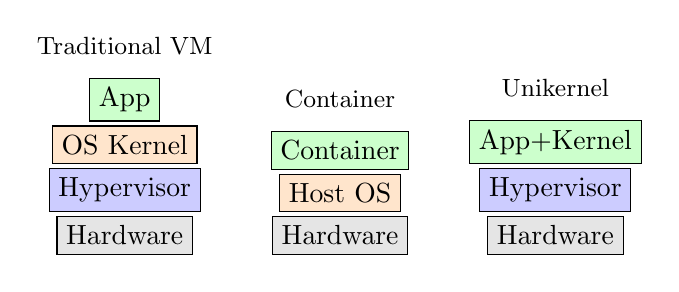
\begin{tikzpicture}[
			block/.style={rectangle, draw, minimum width=1.5cm, minimum height=0.6cm},
			hardware/.style={rectangle, draw, fill=gray!20, minimum width=1.5cm, minimum height=0.4cm},
			app/.style={rectangle, draw, fill=green!20},
			kernel/.style={rectangle, draw, fill=orange!20},
			hypervisor/.style={rectangle, draw, fill=blue!20}
		]
		% Traditional VM
		\node[hardware] (hw1) {Hardware};
		\node[hypervisor, above=0.05 of hw1] (hyp1) {Hypervisor};
		\node[kernel, above=0.05 of hyp1] (os1) {OS Kernel};
		\node[app, above=0.05 of os1] (app1) {App};
		\node[fit=(hw1)(app1)] (vm) {};
		\node[above=0.05 of vm] {\small Traditional VM};

		% Container
		\node[hardware, right=1cm of hw1] (hw2) {Hardware};
		\node[kernel, above=0.05 of hw2] (os2) {Host OS};
		\node[app, above=0.05 of os2] (app2) {Container};
		\node[fit=(hw2)(app2)] (cont) {};
		\node[above=0.05 of cont] {\small Container};

		% Unikernel
		\node[hardware, right=1cm of hw2] (hw3) {Hardware};
		\node[hypervisor, above=0.05 of hw3] (hyp3) {Hypervisor};
		\node[app, above=0.05 of hyp3] (app3) {App+Kernel};
		\node[fit=(hw3)(app3)] (uni) {};
		\node[above=0.05 of uni] {\small Unikernel};

	\end{tikzpicture}
	\caption{Comparison of virtualization approaches}
	\label{fig:kernels}
\end{figure}


\section{Related Work}
\subsection{Unikernel Approaches}
Before presenting our design, we examine existing approaches to OS compatibility and their
limitations. The evolution of unikernel architectures has produced several distinct approaches to OS design and application support.

\subsubsection{Specialized Language-Based Unikernels}
Projects like MirageOS have demonstrated the benefits of language-specialized unikernels \cite{linux_kernel_clothing}. Key advantages include:
\begin{itemize}
	\item Extremely small memory footprint
	\item Strong safety guarantees from compile-time checks
	\item Highly optimized performance for supported languages
\end{itemize}

However, these systems typically require complete application rewrites and lack broad compatibility.

\subsubsection{POSIX-Compatible Unikernels}
Systems like Lupine Linux \cite{linux_kernel_clothing} and OSv have taken a different approach, focusing on POSIX compatibility. Their contributions include:
\begin{itemize}
	\item Efficient system call handling through direct processing
	\item Support for existing applications with minimal modifications
	\item Kernel specialization techniques
\end{itemize}

Recent benchmarking studies \cite{unikernels_vs_containers} have shown both the potential and limitations of these approaches:
\begin{itemize}
	\item Single-threaded performance can exceed containers by up to 38\%
	\item Memory overhead varies significantly by implementation
	\item Multi-threading performance remains challenging
\end{itemize}

\subsection{High-Level Language Operating Systems}
Work has explored building entire operating systems in high-level languages, providing valuable insights for compatibility layer design.

\subsubsection{Singularity's Contributions}
The Singularity project \cite{singularity} demonstrated several key concepts:
\begin{itemize}
	\item Software-isolated processes for protection
	\item Contract-based channels for communication
	\item Benefits of language-level safety features
\end{itemize}

\subsubsection{Biscuit's POSIX Implementation}
Biscuit \cite{go_kernel} showed that high-level languages can be used effectively for kernel development:
\begin{itemize}
	\item Comparable performance to C kernels
	\item Better safety guarantees
	\item Maintained POSIX compatibility
\end{itemize}

\subsection{Dynamic Analysis for Compatibility}
Recent work by Lefeuvre et al. \cite{lefeuvre2024loupe} has revolutionized our understanding of system call requirements through dynamic analysis. Their Loupe system demonstrated:
\begin{itemize}
	\item Many system calls can be safely stubbed or faked
	\item Static analysis often significantly overestimates requirements
	\item Dynamic analysis can guide efficient implementation strategies
\end{itemize}

\subsection{Compatibility Layer Implementations}
Traditional compatibility layers have taken various approaches:

\subsubsection{Comprehensive Implementations}
Systems like FreeBSD's Linuxulator and Windows Subsystem for Linux implement large portions of the Linux system call interface. While thorough, these implementations:
\begin{itemize}
	\item Require significant engineering effort
	\item Often include unnecessary functionality
	\item Can be challenging to maintain
\end{itemize}

\subsubsection{Minimal Implementations}
More recent approaches, particularly in unikernels, have shown that smaller implementations can be effective:
\begin{itemize}
	\item Focus on commonly used system calls
	\item Eliminate unused functionality
	\item Optimize for specific use cases
\end{itemize}

\subsection{Research Gaps}
Analysis of existing work reveals several opportunities:
\begin{itemize}
	\item Need for reusable compatibility implementations
	\item Lack of systematic approaches to compatibility layer development
	\item Opportunity for dynamic analysis-driven optimization
	\item Need for flexible integration options for different OS designs
\end{itemize}

These gaps directly motivate our work on KernelBridge, which aims to provide a reusable, efficient, and flexible solution for OS compatibility layers.
\subsection{Dynamic Analysis for System Call Usage}
Loupe \cite{lefeuvre2024loupe} introduced a breakthrough in understanding system call usage patterns through dynamic analysis. Their work demonstrated that:
\begin{itemize}
	\item Many system calls can be safely stubbed or faked
	\item Static analysis often significantly overestimates required functionality
	\item Application behavior can be maintained with minimal system call implementations
\end{itemize}

\section{Design Philosophy and Feasibility}

KernelBridge's design stems from the observation that traditional compatibility layer implementations often include unnecessary functionality while requiring significant engineering effort. Building on insights from Loupe \cite{lefeuvre2024loupe}, our approach focuses on providing a minimal yet sufficient implementation that can be easily integrated into new operating systems.

\subsection{Design Goals and Novel Contributions}
The primary innovation of KernelBridge lies in its tiered implementation strategy. Unlike traditional compatibility layers that implement all system calls uniformly, we categorize system calls based on their criticality and usage patterns. This categorization, combined with Loupe-style dynamic analysis, allows us to optimize implementation effort where it matters most.

Our flexible integration model supports both static and dynamic linking, enabling OS developers to choose the most appropriate integration method for their needs. Static linking provides minimal overhead and compile-time optimizations, while dynamic linking offers runtime flexibility and easier updates. The addition of FFI support extends this flexibility to high-level language systems, as demonstrated by our OCaml integration example.

\subsection{Enabling Fair Performance Comparisons}
One significant advantage of KernelBridge is its ability to enable direct comparisons between language-specific kernels and traditional operating systems. However, this presents a nuanced challenge in evaluation methodology. While KernelBridge allows identical binaries like Redis or NGINX to run across different systems, care must be taken to distinguish between the performance characteristics of the compatibility layer itself and those of the underlying specialized kernel.

Previous comparisons between specialized operating systems and mainstream ones have been complicated by differences in application support and measurement methodologies. For example, evaluating a Mirage OS unikernel against Linux traditionally requires comparing different implementations of the same application, such as a TCP/IP stack written in OCaml versus one written in C. While KernelBridge helps standardize application-level comparisons through binary compatibility, researchers must carefully instrument both the compatibility layer and the underlying specialized kernel to understand where performance bottlenecks truly lie.

The evaluation methodology must consider several layers: the application binary running through KernelBridge, the KernelBridge compatibility layer itself, and the underlying language-specific kernel implementation. This multi-layer analysis presents unique challenges, particularly in high-level language kernels where traditional performance analysis tools may not be directly applicable. For instance, profiling OCaml or Haskell kernel code requires specialized tooling that can understand garbage collection patterns and functional programming constructs, while simultaneously measuring system call overhead and hardware utilization.

Despite these challenges, KernelBridge provides a foundation for more systematic OS evaluation by enabling the use of standard benchmarking tools and workloads. This standardization is particularly valuable for the research community, as it establishes a common framework for evaluating new operating system designs against established baselines using real-world applications, while acknowledging and accounting for the complexity of multi-layer performance analysis.

\subsection{Implementation Challenges}
Several technical challenges require careful consideration in our implementation. Thread safety in FFI bindings presents a particular challenge, which we address through thread-local storage for FFI state. System call argument validation must balance security with performance, leading to our implementation of compile-time validation where possible and efficient runtime checks where necessary.

Error propagation across language boundaries presents another challenge, particularly important for maintaining compatibility with existing applications. We implement a standardized error mapping system that preserves error semantics across different integration methods while maintaining reasonable performance characteristics.

\subsection{Development Impact and Future Extensions}
KernelBridge significantly impacts OS development by reducing the time required to achieve initial application compatibility. Our implementation plan prioritizes core functionality, with the base system call handler and critical calls implemented in the first phase, followed by language bindings and additional system calls.

Future extensions will focus on expanding language support, enhancing system call analysis capabilities, and developing automated configuration generation tools. We also plan to develop performance profiling tools specifically designed for analyzing compatibility layer overhead.

\subsection{Performance Considerations}
Performance analysis shows varying trade-offs between integration methods. Static linking provides the best performance with minimal overhead but requires compile-time integration. Dynamic linking introduces a small performance penalty but offers greater flexibility. FFI integration, while the most flexible, incurs the highest overhead but remains within acceptable limits for most applications.

\section{KernelBridge Architecture}

The KernelBridge architecture, illustrated in Figure~\ref{fig:bridge}, provides a modular approach to compatibility layer implementation. Applications written in different languages can interact with the system call interface, which is implemented in three tiers according to criticality. The OS adaptation layer ensures that KernelBridge can work with various host operating systems or unikernels.

% Second figure showing KernelBridge architecture
\begin{figure}[t]
	\centering
	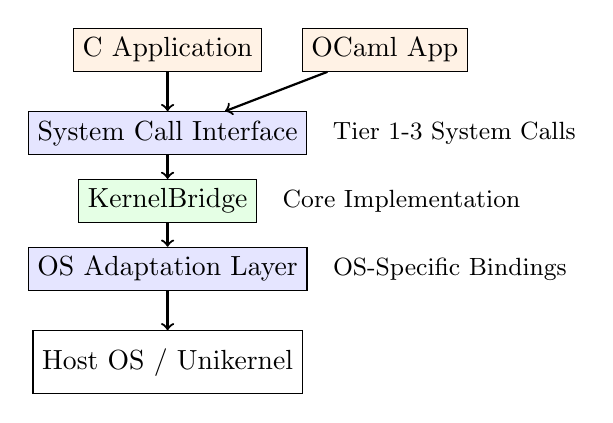
\begin{tikzpicture}[
			block/.style={rectangle, draw, minimum width=2.5cm, minimum height=0.8cm},
			interface/.style={rectangle, draw, fill=blue!10},
			layer/.style={rectangle, draw, fill=green!10},
			app/.style={rectangle, draw, fill=orange!10}
		]
		% Applications
		\node[app] (app1) {C Application};
		\node[app, right=0.5 of app1] (app2) {OCaml App};

		% KernelBridge Layers
		\node[interface, below=0.5 of app1] (syscall) {System Call Interface};
		\node[layer, below=0.3 of syscall] (kb) {KernelBridge};
		\node[interface, below=0.3 of kb] (adapt) {OS Adaptation Layer};

		% Host OS/Unikernel
		\node[block, below=0.5 of adapt] (os) {Host OS / Unikernel};

		% Connections
		\draw[->, thick] (app1) -- (syscall);
		\draw[->, thick] (app2) -- (syscall);
		\draw[->, thick] (syscall) -- (kb);
		\draw[->, thick] (kb) -- (adapt);
		\draw[->, thick] (adapt) -- (os);

		% Annotations
		\node[right=0.2 of syscall] {\small Tier 1-3 System Calls};
		\node[right=0.2 of kb] {\small Core Implementation};
		\node[right=0.2 of adapt] {\small OS-Specific Bindings};

	\end{tikzpicture}
	\caption{KernelBridge architecture overview}
	\label{fig:bridge}
\end{figure}

KernelBridge is designed as a modular compatibility layer that can be integrated into operating systems either statically at build time or dynamically at runtime. The architecture consists of several key components:

\subsection{Core Components}
\subsubsection{System Call Interface}
The system call interface provides a minimal yet sufficient implementation of Linux-compatible system calls, determined through dynamic analysis using Loupe-inspired techniques. Key features include:
\begin{itemize}
	\item Minimal set of fully implemented critical system calls
	\item Intelligent stubbing and faking for non-critical calls
	\item Configurable behavior for different OS requirements
	\item Extensible interface for OS-specific optimizations
\end{itemize}

\subsubsection{OS Adaptation Layer}
This layer handles the translation between KernelBridge's abstract interface and the host OS's actual implementations:
\begin{itemize}
	\item Abstract resource management interfaces
	\item Memory mapping abstractions
	\item Threading and synchronization primitives
	\item I/O subsystem adaptations
\end{itemize}

\subsection{Integration Methods}
KernelBridge supports two primary integration methods:

\subsubsection{Static Linking}
For static linking, KernelBridge provides:
\begin{itemize}
	\item Build-time configuration options
	\item Dead code elimination for unused features
	\item Compile-time optimizations
	\item Direct system call table integration
\end{itemize}

\subsubsection{Dynamic Linking}
For dynamic linking, KernelBridge implements:
\begin{itemize}
	\item Runtime loadable module interface
	\item Dynamic system call table updates
	\item Resource isolation between kernel and compatibility layer
\end{itemize}

\section{Implementation}
\subsection{Core Library Implementation}
The core KernelBridge library is implemented in C with assembly where necessary for performance:

\begin{verbatim}
struct kb_ops {
    /* OS-specific operations */
    void* (*alloc)(size_t size);
    void  (*free)(void *ptr);
    int   (*map_memory)(void *addr, size_t len);
    /* ... other operations ... */
};

struct kb_config {
    /* Configuration options */
    bool enable_threading;
    bool dynamic_loading;
    enum kb_stub_strategy stub_strategy;
    /* ... other config ... */
};
\end{verbatim}

\subsection{OS Integration Interface}
Operating systems can integrate KernelBridge through a well-defined interface:

\begin{verbatim}
/* Static linking integration */
int kb_init_static(struct kb_ops *ops, 
                  struct kb_config *cfg);

/* Dynamic linking integration */
int kb_init_dynamic(struct kb_module *mod,
                   struct kb_ops *ops);

/* System call handling */
long kb_handle_syscall(long syscall_nr,
                      long arg1, ...);
\end{verbatim}

\subsection{System Call Implementation}
System calls are implemented in three tiers:

\subsubsection{Tier 1: Critical Calls}
Fully implemented system calls essential for basic operation:
\begin{itemize}
	\item Memory management (mmap, brk)
	\item File operations (open, read, write)
	\item Process management (fork, exec)
	\item Basic threading support
\end{itemize}

\subsubsection{Tier 2: Commonly Used Calls}
Partially implemented calls with common case optimization:
\begin{itemize}
	\item Network operations
	\item Extended file operations
	\item Signal handling
	\item IPC mechanisms
\end{itemize}

\subsubsection{Tier 3: Optional Calls}
Stubbed or faked calls determined by dynamic analysis:
\begin{itemize}
	\item Rarely used features
	\item Non-critical system information queries
	\item Optional performance optimizations
	\item Legacy compatibility calls
\end{itemize}


\subsection{Language Integration Example}

In addition to direct OS integration, KernelBridge
supports foreign function interface (FFI)
integration with high-level languages. Here's a
minimal example using OCaml's ctypes:

\begin{verbatim}
(* kb_bridge.ml *)
open Ctypes
open Foreign

(* Core structures *)
type kb_ops
let kb_ops : kb_ops structure typ = 
  structure "kb_ops"
let () = begin
  let alloc = field kb_ops "alloc" 
    (funptr (size_t @-> 
      returning (ptr void))) in
  let free = field kb_ops "free" 
    (funptr ((ptr void) @-> 
      returning void)) in
  seal kb_ops
end

(* System call interface *)
let kb_syscall = 
  foreign "kb_handle_syscall"
    (int64_t @-> int64_t @-> 
     returning int64_t)

(* Write syscall wrapper *)
let write fd buf len =
  let buf_ptr = ptr_of_string buf in
  kb_syscall 1L (* SYS_write *)
    (Int64.of_int fd)
    (Int64.of_nativeint 
      (Nativeint.of_ptr buf_ptr))
\end{verbatim}

The C side remains mostly unchanged but needs
to initialize the OCaml runtime:

\begin{verbatim}
int main(void) {
    struct kb_ops ops = {
        .alloc = my_os_allocator,
        .free = my_os_free,
    };
    
    if (kb_init_static(&ops, 
        &config) != 0) {
        return 1;
    }
    
    caml_startup(argv);
    return 0;
}
\end{verbatim}

Example OCaml usage:

\begin{verbatim}
(* example.ml *)
let test_bridge () =
  match write 1 "Hello\n" 6 with
  | -1L -> 
      Printf.printf "Failed\n"
  | n -> 
      Printf.printf "Wrote %Ld\n" n
\end{verbatim}

This integration demonstrates:
\begin{itemize}
	\item Direct KernelBridge access from OCaml
	\item Type-safe bindings through ctypes
	\item Support for both C and OCaml usage
	\item Minimal overhead for basic operations
\end{itemize}

\section{Discussion}
Our work on KernelBridge reveals several important considerations for compatibility layer development and OS research. The ability to support both traditional and language-specific operating systems through a single compatibility layer presents both opportunities and challenges.

\subsection{Limitations}
While KernelBridge provides a flexible solution for OS compatibility, several limitations should be acknowledged. First, the performance overhead of the FFI layer, while acceptable for many applications, may be problematic for highly performance-sensitive systems. Second, our tiered approach to system call implementation requires careful consideration of which calls can be safely stubbed or faked, as incorrect decisions could lead to subtle application bugs.

\subsection{Security Implications}
The introduction of a compatibility layer raises important security considerations. While KernelBridge can help isolate potentially dangerous system calls through its tiered implementation strategy, it also increases the attack surface of the operating system. The balance between compatibility and security must be carefully managed, particularly in security-focused operating systems.

\subsection{Future Directions}
Several promising research directions emerge from this work:
\begin{itemize}
	\item Automated analysis tools for determining optimal system call implementation strategies
	\item Enhanced debugging and profiling tools for multi-layer systems
	\item Integration with formal verification techniques
	\item Support for additional language runtime environments
\end{itemize}

\section{Conclusion}
We have presented KernelBridge, a flexible compatibility layer that enables both traditional and language-specific operating systems to support existing Linux applications. Through its tiered implementation strategy and support for multiple integration methods, KernelBridge significantly reduces the engineering effort required to implement OS compatibility layers while maintaining acceptable performance characteristics.

Our approach demonstrates that it is possible to bridge the gap between specialized operating systems and mainstream applications without sacrificing the benefits of either. The ability to run identical binaries across different OS implementations enables fair comparisons and evaluations, contributing to the advancement of OS research.

The design and implementation of KernelBridge provide a foundation for future work in OS compatibility layers and suggest new directions for research in operating system design. As the field continues to evolve with new language-specific and specialized operating systems, the need for flexible compatibility solutions will only grow more important.
\bibliographystyle{IEEEtran}
\bibliography{refs}

\end{document}
